\chapter{Validation of the model}\label{Australiano}

To check the reliability of the model, we simulated the HPV vaccination campaign carried out in Australia \cite{ali2013genital}, and compared them with the actual impact published \cite{ali2013genital}. In 2007, Australian health authorities started a vaccination program for 12--13 year-old girls with a~coverage of $73\%$ ($83\%$ in the first dose, $80\%$ in the second dose and $73\%$ in the third dose). In addition, from 2007 to 2009, there was a catch-up vaccination program for women aged 13--26 with a decreasing coverage with age until $52\%$ in women aged 20--26. Their results can be summarized as follows \cite{ali2013genital}:

\begin{itemize}
	\item Two years after the vaccine was introduced, the proportion of genital warts diagnosed declined by a $59\%$ in vaccine eligible young women aged 12--26 years in $2007$, and by $39\%$ in men of the same age.
	\item No significant decline was observed in women or men older than $26$ years old, non-resident young women, or men who have sex with men.
\end{itemize}

As in \cite{DezDomingo2017}, two different scenarios were considered to be simulated:

\begin{itemize}
	\item Scenario 1: vaccination of $83\%$ of the $14$ year-old girls (or younger girls) plus a catch-up with coverage $73\%$ for 14--26 year-old women.
	\item Scenario 2: vaccination of $73\%$ of $14$ year-old girls (or younger girls) plus a catch-up with a~vaccination coverage of $52\%$ for 14--26 year-old women.
\end{itemize}

These simulations represented the upper and lower bounds of the scenario implemented in Australia. 

\section{How to measure the decline}\label{sec:decline}
We call $I$ the number of infected women/men/MSM of HPV just before the starting of the vaccination campaign; we call $V = ( v_1, \ldots, v_N)$ to the number of infected women/men/MSM of HPV every month from the starting of the vaccination program until the end of the simulation. Then, the vector 

\begin{equation}
100 \times \left( 1-\displaystyle\frac{v_1}{I}, \ldots, 1-\displaystyle\frac{v_N}{I} \right) \; 
\label{formula:decline}
\end{equation}

is a measure of the percentage of decline of number of infected women/men/MSM of HPV after the beginning of the vaccination campaign. We can apply this procedure to find out the decline of LR HPV or HR HPV infected people.

Also, we should note that if a fixed proportion of LR HPV infected individuals develops genital warts, then the expression of the decline given by \eqref{formula:decline} may be an estimation of the decline of genital warts cases, taking into account the natural delay between the infection and the apparition of the warts. Analogously, it would be valid for HR HPV infected individuals and the cancer cases. 

\section{Does our model return similar values to those in \cite{ali2013genital}?}
In this section, we are going to show figures about prevalence or decline of the percentage of women, men and MSM infected of LR 6/11, the HPV type responsible of $90\%$ of genital warts. Taking into account that genital warts, in average, use to appear 6 months after the infection, the figures about prevalence or decline will be a good estimation of the prevalence and the  decline of genital warts.  

Figure \ref{fig:prev_AUS_6_11} shows the percentage of women, men and MSM aged 14–26 infected of LR 6/11 after starting the vaccination program in both simulated scenarios. We can see the fast decrease for women and men in both scenarios from the very beginning. MSM, in average, have a slow decreasing. 

\begin{figure}[!]
	\centering
	\begin{tabular}{cc}
		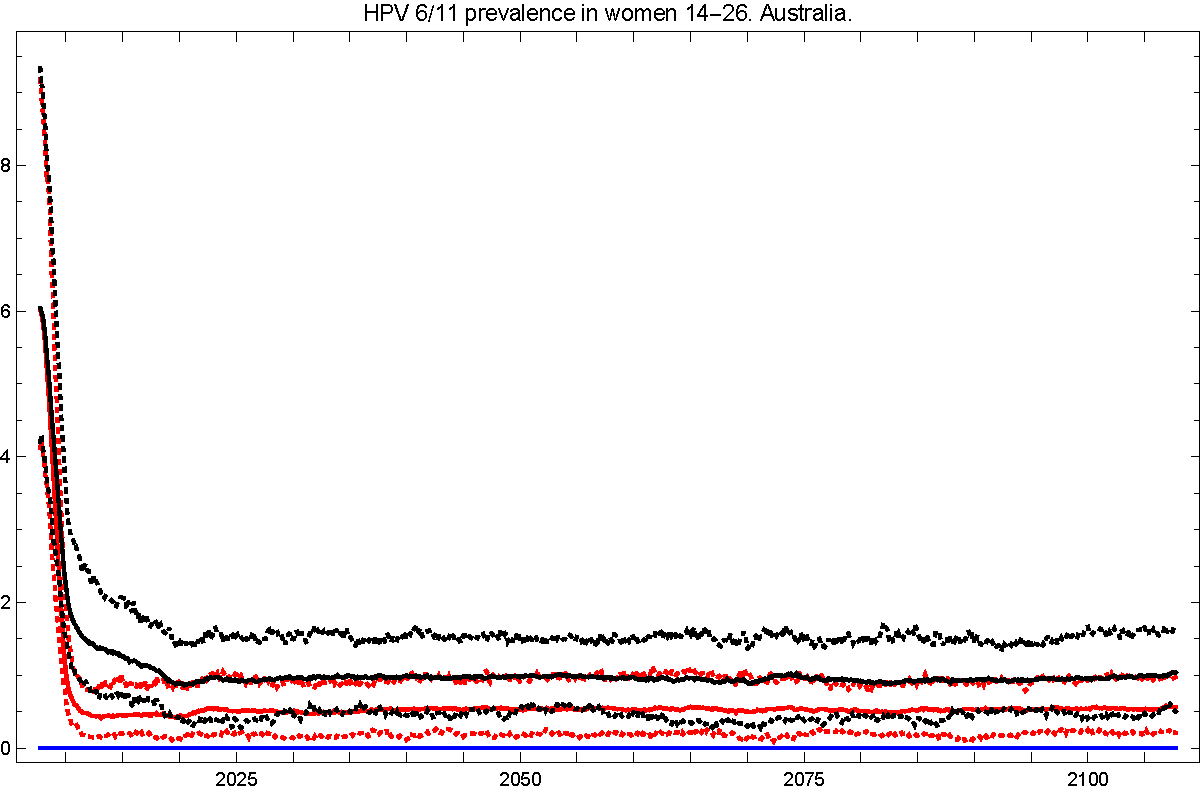
\includegraphics[width=0.5\linewidth]{IMGs/3.-Australia/Retr_muj_14_26_verr_Australia.pdf}	& 
		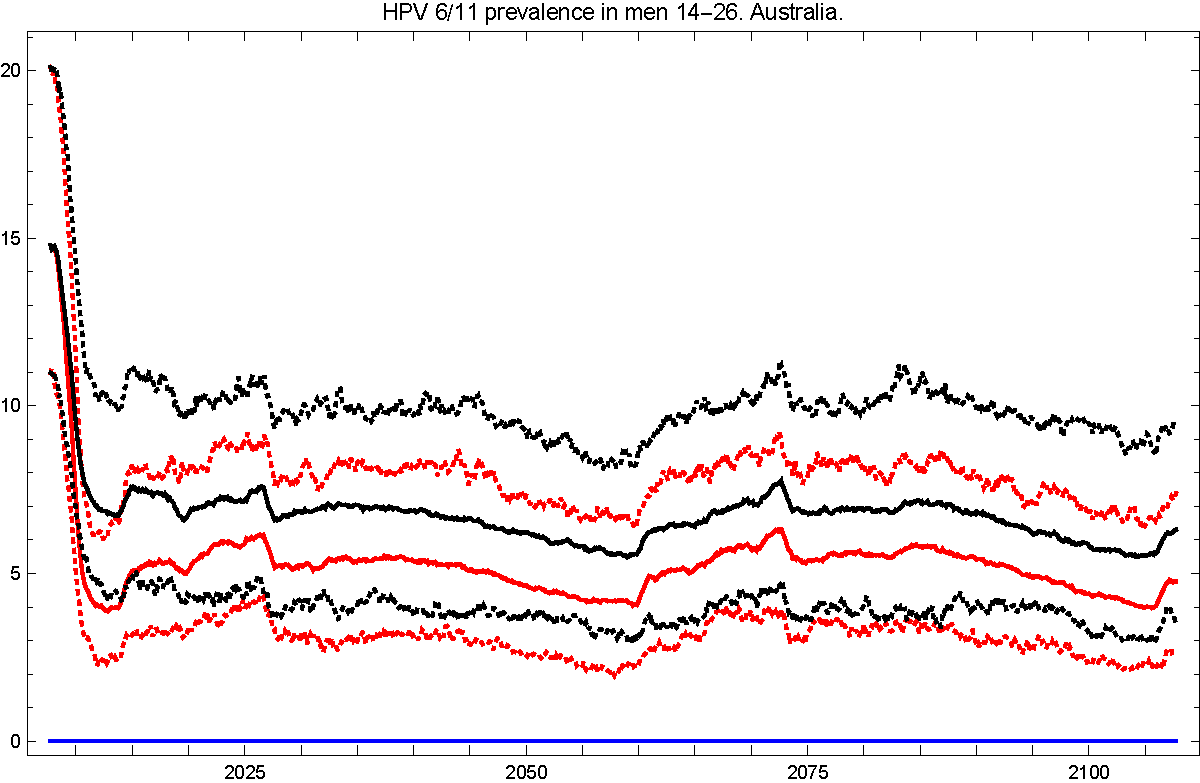
\includegraphics[width=0.5\linewidth]{IMGs/3.-Australia/Retr_hom_14_26_verr_Australia.pdf}  \\ 
		(a)	& (b) \\ 
		\multicolumn{2}{c}{ 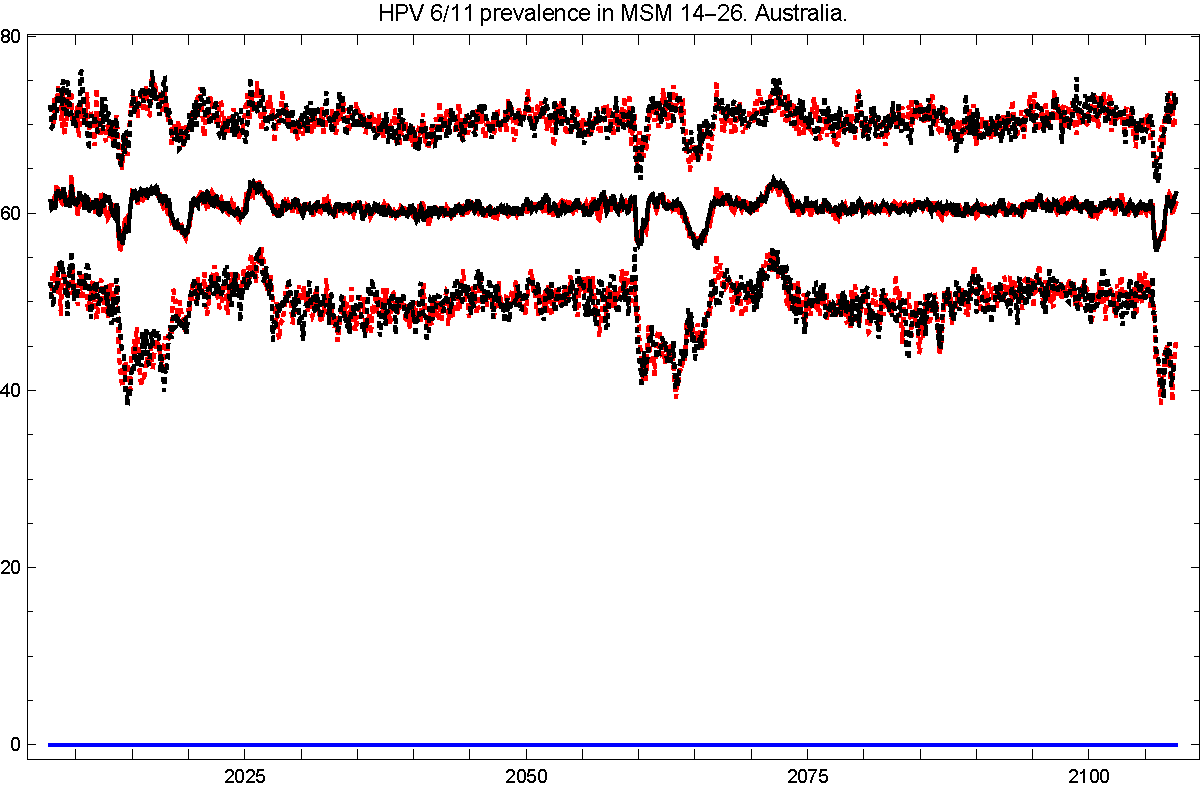
\includegraphics[width=0.5\linewidth]{IMGs/3.-Australia/Retr_MSM_14_26_verr_Australia.pdf} } \\ 
		\multicolumn{2}{c}{(c)} \\ 
	\end{tabular} 
	\caption{Percentage of women (a), men (b) and MSM (c) aged 14–26 infected of LR HPV 6 and/or 11 after the implementation of the vaccination program. The red lines correspond to the average and $95\%$ confidence interval for Scenario 1 and the black lines to Scenario 2.  We can see the fast decrease for women and men in both scenarios from the very beginning. However, there is not effect on MSM.}
	\label{fig:prev_AUS_6_11}	
\end{figure}

In Figure \ref{fig:decline_AUS_6_11}, we have plotted the same data as in Figure \ref{fig:prev_AUS_6_11} but from another point of view: the average percentage of decline of women and men infected of LR HPV 6 and/or 11. As the vaccination program progresses over time, the percentage of decline obviously grows. After 2 years, the model shows a decline of

\begin{itemize}
	\item Scenario 1: $72.0\%$ with CI $95\%$ $[67.7\%, 76.5\%]$ for women and $38.9\%$ with CI $95\%$ $[32.0\%, 45.5\%]$ for men. 
	\item Scenario 2: $54.8\%$ with CI $95\%$ $[48.5\%, 59.0\%]$ for women and $27.7\%$ with CI $95\%$ $[21.3\%, 34.5\%]$ for men. 
\end{itemize}

Australian reported levels of decline ($59\%$ in women and $39\%$ in men aged 14-26) will be reached by the model after

\begin{itemize}
	\item Viruses, 9(10):30 years with CI $95\%$ $[1.5, 1.75]$ for women and $2.0$ years with CI $95\%$ $[1.75, 2.16]$ for men,
	\item Scenario 2: $2.1$ years with CI $95\%$ $[2.0, 2.33]$ for women and $2.42$ years with CI $95\%$ $[2.08, 2.83]$ for men.
\end{itemize}

\begin{figure}[!]
	\centering
	\begin{tabular}{cc}
		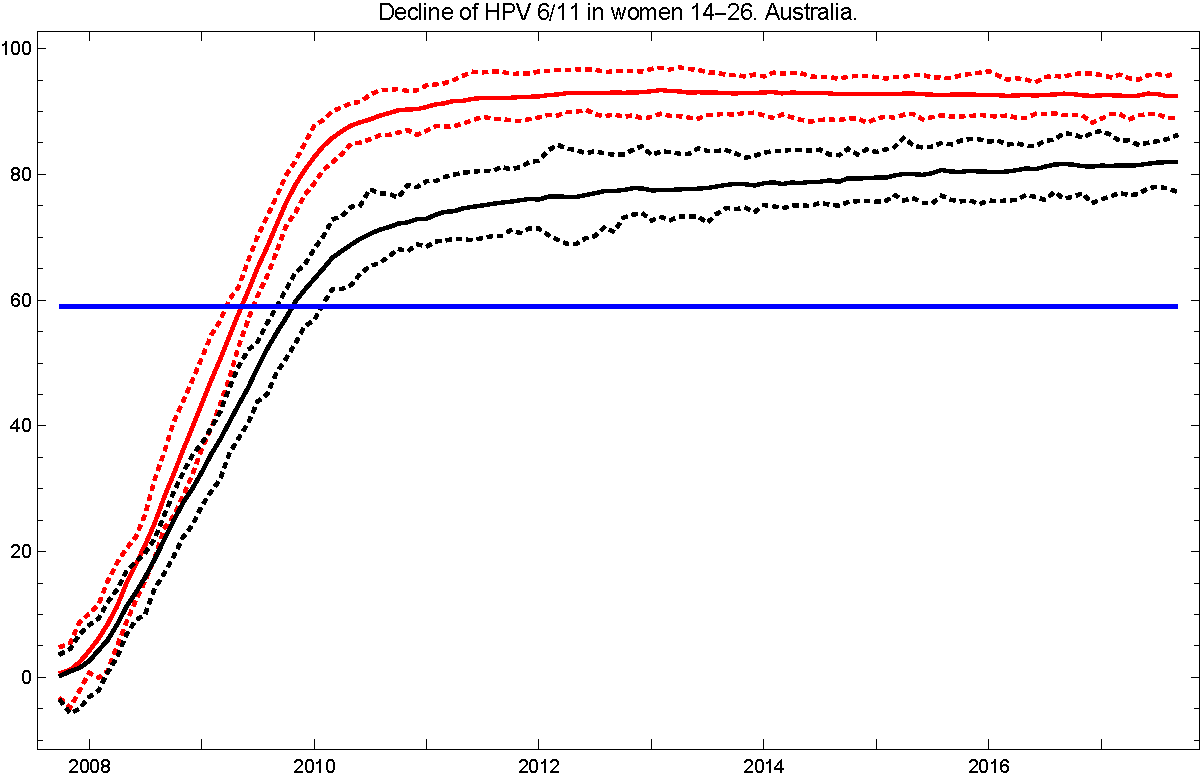
\includegraphics[width=0.5\linewidth]{IMGs/3.-Australia/Decl_muj_14_26_verr_Australia.pdf}	& 
		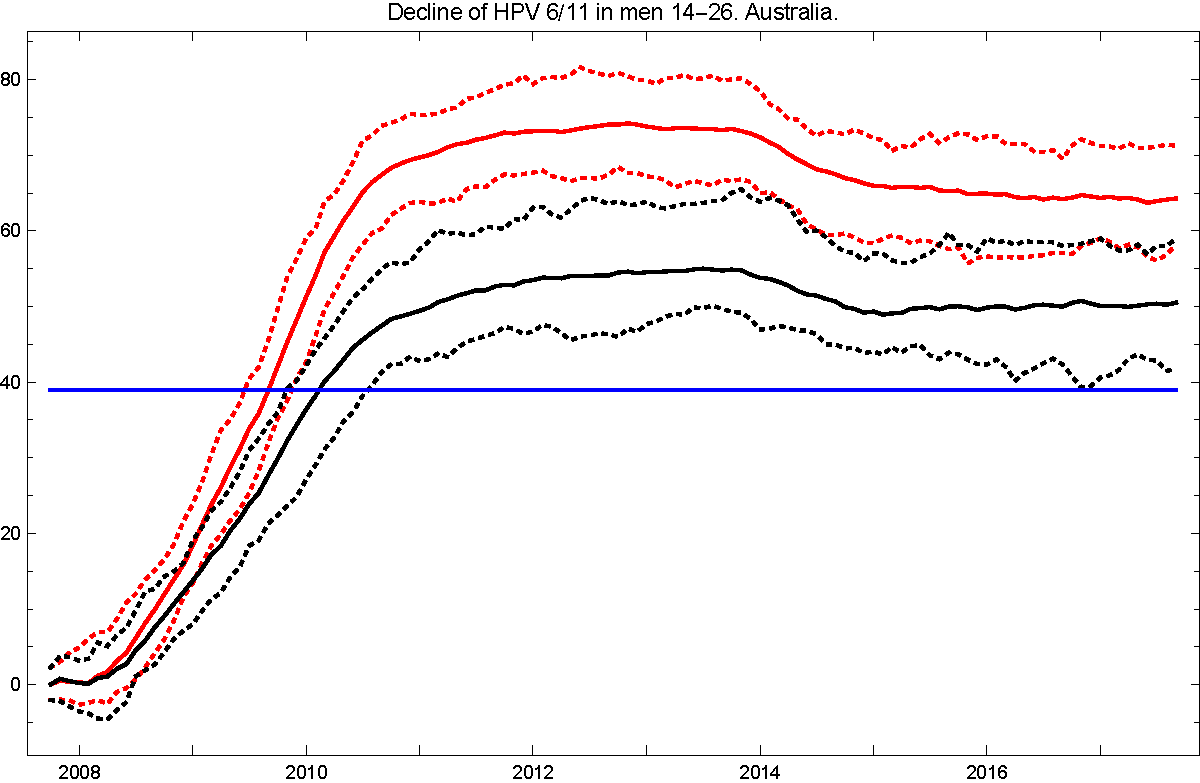
\includegraphics[width=0.5\linewidth]{IMGs/3.-Australia/Decl_hom_14_26_verr_Australia.pdf}  \\ 
		(a)	& (b) 
	\end{tabular} 
	\caption{Percentage of decline of women (a) and men (b) aged 14–26 infected of LR HPV 6 and/or 11 (and consequently of genital warts) after the implementation of the vaccination program. The red lines correspond to the average and $95\%$ confidence interval for Scenario 1 and the black lines to Scenario 2. After 2 years, the model shows a decline of $72\%$ for Scenario 1 and $54.8\%$ for Scenario 2, in average, for women and $38.9\%$ for Scenario 1 and $27.7\%$ for Scenario 2, in average, for men.}
	\label{fig:decline_AUS_6_11}
\end{figure}

No significant impact on the rate of infection was observed in men aged 27–64 and women 2 years after the implementation of the vaccination program (Figure \ref{fig:decline_AUS_6_11_27_64}) and the same in women agreeing the observations reported in \cite{ali2013genital}. It can be explained by the fact that, usually, individuals have sexual intercourses with people more or less the same age.

Then, our model predict figures close to the ones given in \cite{ali2013genital}.

\begin{figure}[!]
	\centering
	\begin{tabular}{cc}
		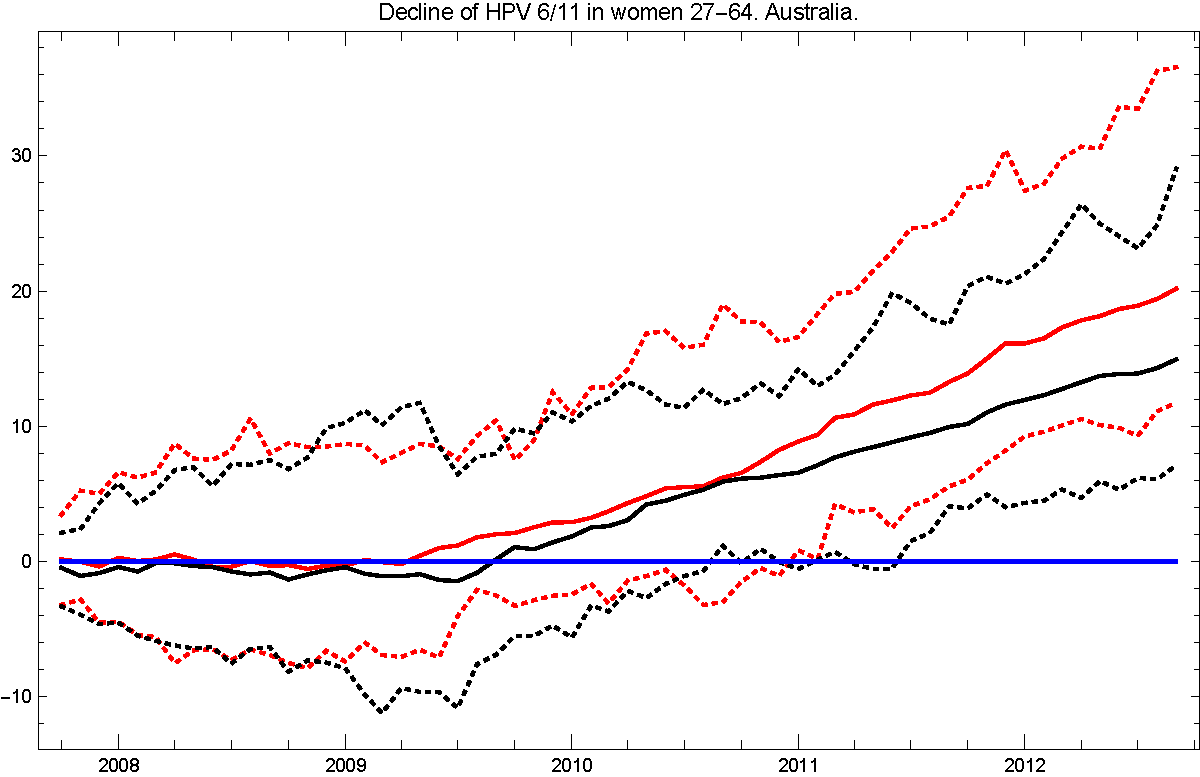
\includegraphics[width=0.5\linewidth]{IMGs/3.-Australia/Decl_muj_27_64_verr_Australia.pdf}	& 
		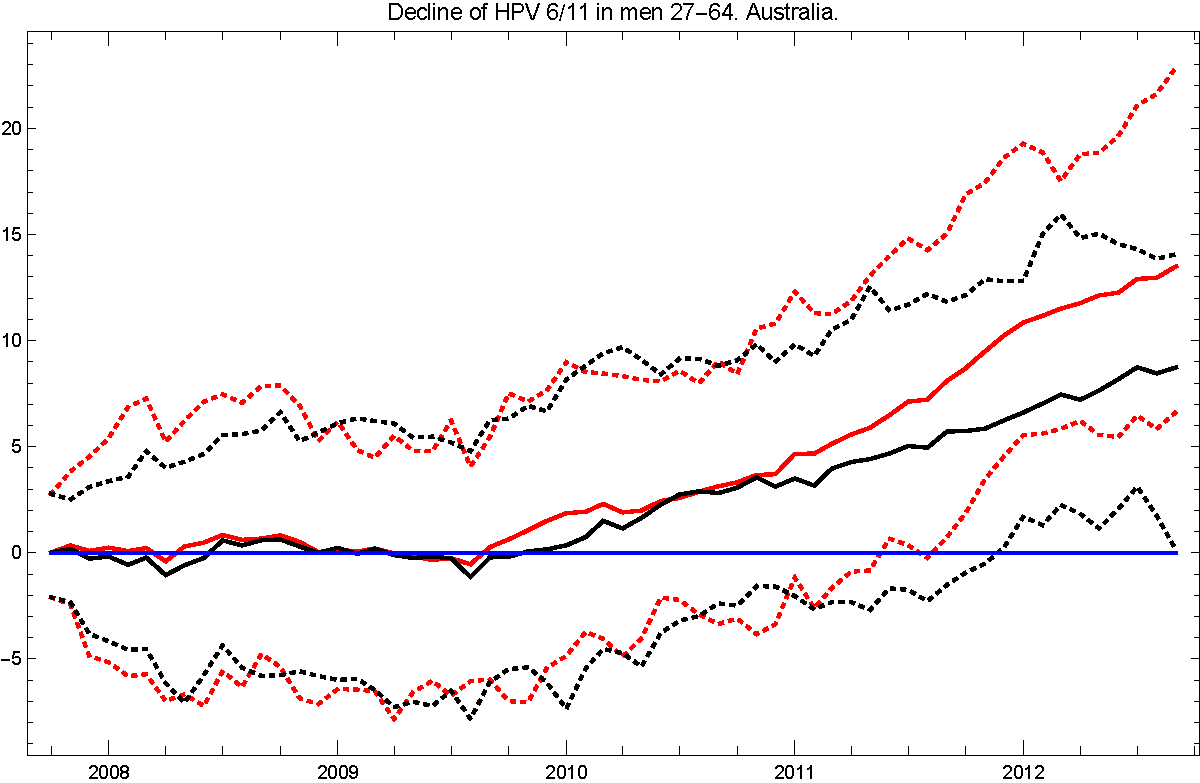
\includegraphics[width=0.5\linewidth]{IMGs/3.-Australia/Decl_hom_27_64_verr_Australia.pdf}  \\ 
		(a)	& (b) 
	\end{tabular} 
	\caption{Percentage of decline of women (a) and men (b) aged 27–64 infected of LR HPV 6 and/or 11 (and consequently of genital warts) after the implementation of the vaccination program in both scenarios. The red lines correspond to the average and $95\%$ confidence interval for Scenario 1 and the black lines to Scenario 2. Notice that, in average, no significant decline appears in the 5 years after the implementation of the vaccination program.}
	\label{fig:decline_AUS_6_11_27_64}
\end{figure}

\section{Study of the herd immunity effect over HPV LR infection}
The herd immunity effect in both scenarios is shown in Figure \ref{fig:decline_AUS_6_11_14_64} for women, men and MSM. Notice that, in men and MSM, any decline is due to herd immunity. The decline in the whole female population appears when the lines representing their decline are over the vaccination lines (green for Scenario 1 and orange for Scenario2) also shown in this figure. We see that the herd immunity effect starts after 

\begin{itemize}
	\item for women
	\begin{itemize}
		\item Scenario 1: $0.58$ years with CI95\% $[0.0, 22.1]$.
		\item Scenario 2: $0.58$ years with CI95\% $[0.0, 22.1]$.
	\end{itemize}
	\item for men
	\begin{itemize}
		\item Scenario 1: $0.0$ years with CI95\% $[0.0,0.83]$.
		\item Scenario 2: $0.0$ years with CI95\% $[0.0,0.83]$.	
	\end{itemize}
\end{itemize}

The herd immunity effect starts very quickly for men. For MSM, there is not a clear herd immunity effect because the decline is stable over the time. For women, we can see that, practically, the CI$95\%$ decline lines are over the vaccination lines in both scenarios. This means that, in the worst case, only the vaccinated women will be protected and in the best case, almost all women will be protected by vaccination or by herd immunity effect.

\begin{figure}[!]
	\centering
	\begin{tabular}{cc}
		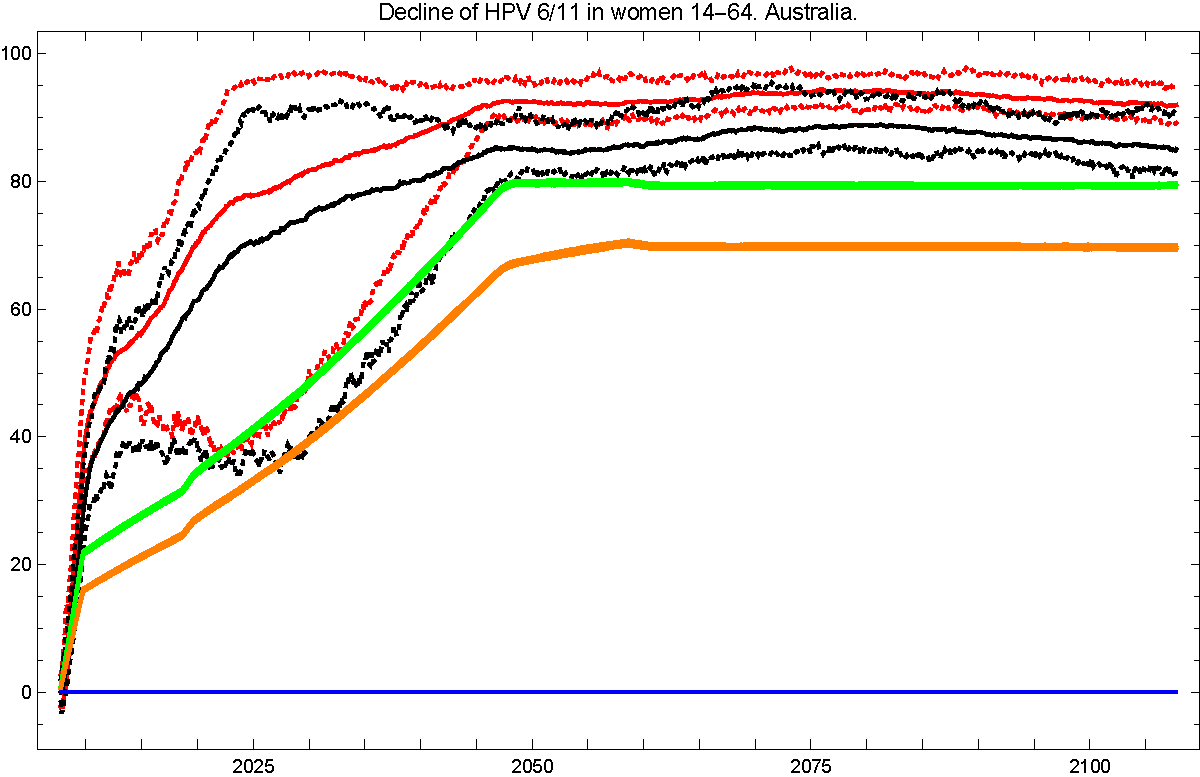
\includegraphics[width=0.5\linewidth]{IMGs/3.-Australia/Decl_muj_14_64_verr_Australia.pdf}	& 
		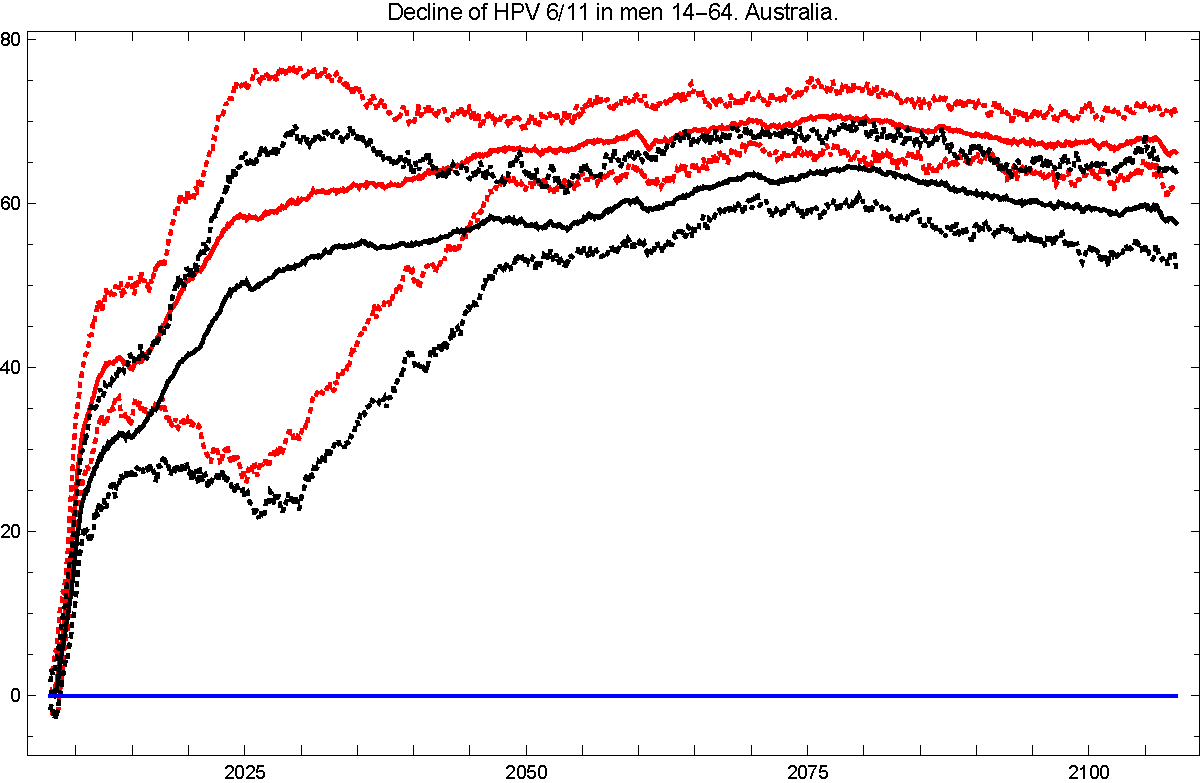
\includegraphics[width=0.5\linewidth]{IMGs/3.-Australia/Decl_hom_14_64_verr_Australia.pdf}  \\ 
		(a)	& (b) \\ 
		\multicolumn{2}{c}{ 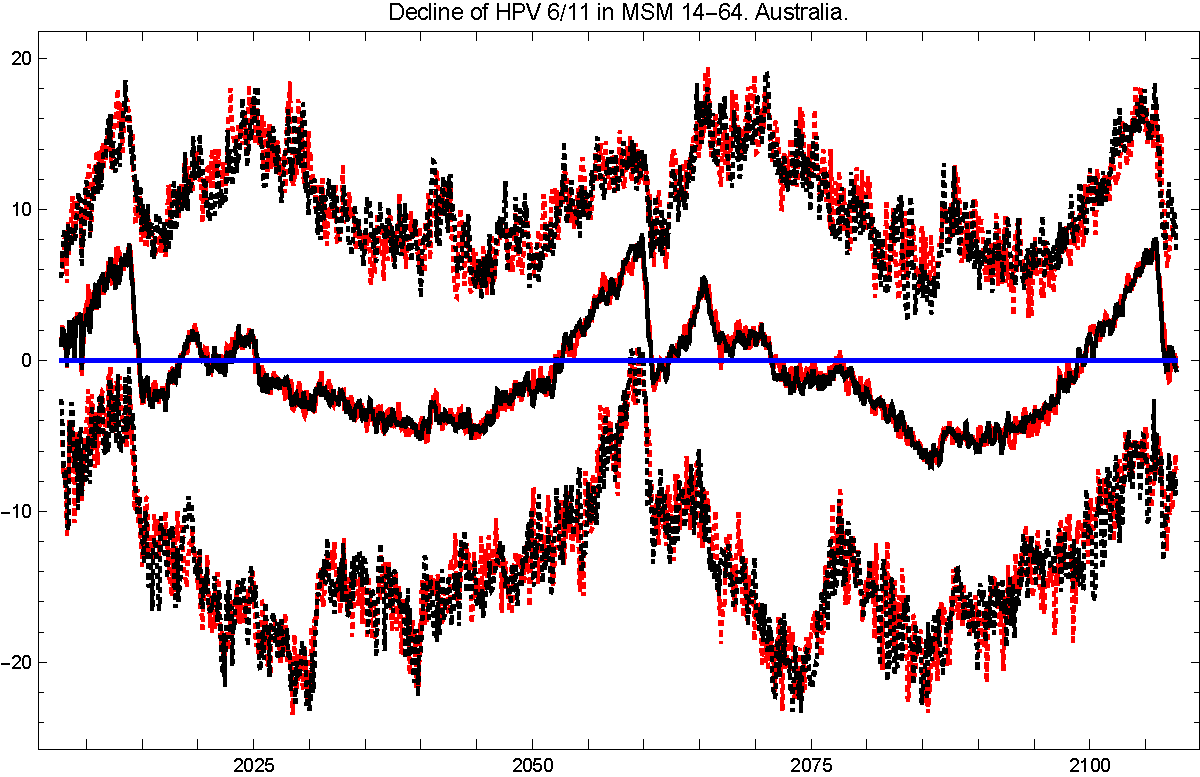
\includegraphics[width=0.5\linewidth]{IMGs/3.-Australia/Decl_MSM_14_64_verr_Australia.pdf} } \\ 
		\multicolumn{2}{c}{(c)} \\ 
	\end{tabular} 
	\caption{Percentage of decline of women (a), men (b) and MSM (c) aged 14-64 for the vaccination program in Australia. The red lines correspond to the average and $95\%$ confidence interval for Scenario 1 and the black lines to Scenario 2. In the figure (a), green and orange lines correspond to women vaccination percentage for Scenario 1 and 2 respectively. Notice that the herd immunity effect contributes to the decline in the number of infections in men and the decline in the number of infections for unvaccinated women. This latter can be seen when the decline lines are over the vaccination line. However, any herd immunity effect can be seen in MSM.}
	\label{fig:decline_AUS_6_11_14_64}
\end{figure}

Notice that the herd immunity effect is very clear within the CI$95\%$ both for women and men, but it does not appear in the MSM population. In the best case scenario, the MSM subpopulation achieves a constant protection level of $10\%-15\%$. This could be attributed to the way in which the MSM individuals are connected: with a very large number of LSPs among them and some casual links with women with large LSPs.